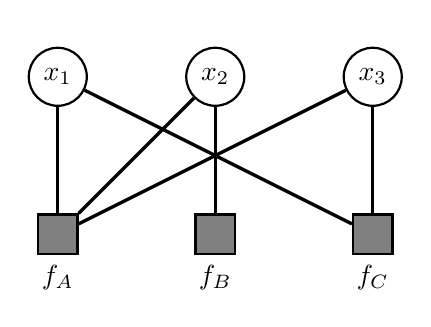
\begin{tikzpicture}[
every edge/.style = {draw=black,very thick},
 vrtx/.style args = {#1/#2}{%
      circle, draw, thick, fill=white,
      minimum size=5mm, label=#1:#2},
 factor/.style args = {#1/#2}{%
      rectangle, draw, thick, fill=gray,
      minimum size=5mm, label=#1:#2}
                    ]
\node(x1) [vrtx=/] at (0, 1) {$x_1$};
\node(fA) [factor=south/$f_A$] at (0,-1) {};
\node(x2) [vrtx=/] at (2, 1) {$x_2$};
\node(fB) [factor=south/$f_B$] at (2,-1) {};
\node(x3) [vrtx=/] at (4, 1) {$x_3$};
\node(fC) [factor=south/$f_C$] at (4,-1) {};
%
\path   (x1)  edge (fA);
\path   (x2)  edge (fB);
\path   (x1)  edge (fC);
\path   (x3)  edge (fC);
\path   (x3)  edge (fA);
\path   (x2)  edge (fA);
\end{tikzpicture}
